% !TEX root = ../main.tex

\chapter{跨环节分析}
\label{chap:analysis}

\section{各段的量级}

表~\ref{tab:segments} 把各段的额定值和主导动态放在一起：功率从 50~kW 跨到 59.6~MW，电流从 500~A 跨到 39.7~kA。联合模型的负载等级与实验四相同，平台段只有约 1~MW，所以交流母线几乎不受影响（电压 1.00005~pu）。联合仿真验证的是链路的拓扑、接口和控制配合，还不能代替对满功率工况的评估。

\begin{dtable}{htbp}{各段的额定值、时间常数与被控量}
\label{tab:segments}
\begin{tabularx}{\linewidth}{P{0.15\linewidth}P{0.25\linewidth}P{0.19\linewidth}P{0.13\linewidth}L}
\toprule
\headrow 环节 & 额定 & 主导时间常数 & 被控量 & 主要非理想性 \\
\midrule
\textcolor{segbus}{\textbf{10~kV 母线}} & 10~kV，短路容量 100~MVA & $\tau_Q=20$~ms，$\tau_E=50$~ms & 母线电压 & 电网阻抗压降 \\
\textcolor{segrect}{\textbf{CS 整流}} & 1.5~kV，39.7~kA，59.6~MW & $L\sub{eq}/R\sub{eq}=3$--$40$~s & 直流电压 & 换相重叠、300~Hz 纹波 \\
\textcolor{seghb}{\textbf{H 桥}} & 2200~V，500~A，50~kW & $L/R=100$~ms & 负载电流 & 死区、开关纹波 \\
\textcolor{segpl}{\textbf{等离子体}} & 100~V，10~kA，1~MW & $L_{\sigma,\mathrm{eq}}/R\sub{p}=12$--$17$~ms & 等离子体电流、磁链 & 回路纹波、磁链消耗 \\
\textbf{整机模型} & 2200~V 母线，约 1.13~MW & 同上 & 母线电压、$i\sub{p}$ & 上述各项的耦合 \\
\bottomrule
\end{tabularx}
\end{dtable}

\section{满功率工况下的母线能力}

实验一的整流器峰值 59.6~MW 能否接到实验二的母线上，是单独任何一个模型都无法回答的问题。

折算到交流侧：六脉波桥二次侧线电流有效值约 $0.816I_d=32.4$~kA，一次侧按变比折算为 3.89~kA，视在功率 67.4~MVA，略小于变压器额定 70~MVA。其中有功 59.6~MW，基波无功约 24~Mvar（对应 $\alpha\approx22^\circ$），基波视在功率 64.4~MVA，其余约 20~MVA 是 5、7、11 次等谐波形成的畸变功率。

短路比为
\begin{equation}
\mathrm{SCR}=\frac{S\sub{sc}}{P}=\frac{100}{59.6}=1.68,
\end{equation}
低于通常作为弱交流系统分界的 3\cite{ieee1204}。沿用第 \ref{chap:bus} 章的相量关系，维持母线 1.0~pu、负载 59.6~MW 和基波无功 24~Mvar 时，以 $S\sub{sc}$ 为基准有
\begin{equation}
E\sub{req}=\Bigl|V+\frac{P-\mathrm{j}Q}{V}\,z_g\Bigr|=1.455\ \mathrm{pu},
\end{equation}
远超 1.15~pu 的限幅。降低母线电压并不能缓解：$V$ 由 1.0~pu 降到 0.8~pu，$E\sub{req}$ 只由 1.455~pu 降到 1.411~pu，因为电压越低电流越大。即使把无功完全补偿，$E\sub{req}$ 仍为 1.261~pu。

结论是这条 100~MVA 母线送不出 59.6~MW，限制来自短路容量而不是控制器。图~\ref{fig:scr}(a) 和表~\ref{tab:scr} 给出 $E\sub{req}$ 随短路容量的变化：约 270~MVA 时 $E\sub{req}$ 降到 1.15~pu，取 300~MVA（SCR $\approx5$）时为 1.132~pu。这一结果与实验二自身的重载工况一致：19.3~MW 时 $E$ 已顶到 1.15~pu，母线掉到 0.879~pu。真实装置中，CS 整流器需要接到短路容量更大的母线上，或配置无功补偿和调压手段。

\begin{figure}[htbp]
\centering
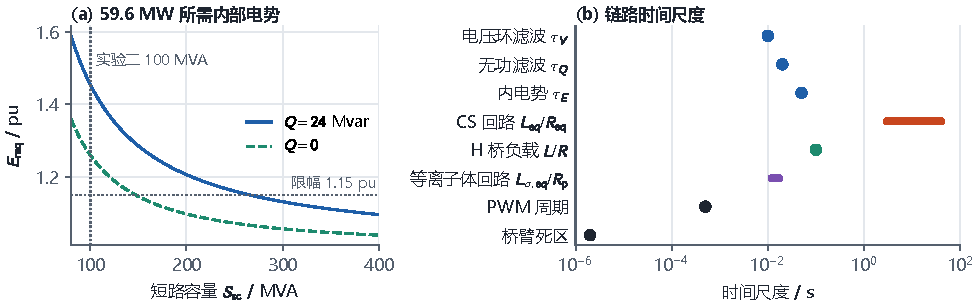
\includegraphics[width=\linewidth]{analysis_scr_time}
\caption{(a) 维持 59.6~MW 所需内部电势随短路容量的变化，(b) 链路各环节的时间尺度，颜色对应图~\ref{fig:chain} 的环节}
\label{fig:scr}
\end{figure}

\begin{dtable}{htbp}{短路容量与维持 59.6~MW 所需的内部电势}
\label{tab:scr}
\begin{tabularx}{\linewidth}{LRRRRR}
\toprule
\headrow $S\sub{sc}$ / MVA & 100 & 200 & 250 & 300 & 350 \\
\midrule
SCR & 1.7 & 3.4 & 4.2 & 5.0 & 5.9 \\
$E\sub{req}$ / pu & 1.455 & 1.206 & 1.161 & 1.132 & 1.111 \\
\bottomrule
\end{tabularx}
\end{dtable}

\section{时间尺度}

图~\ref{fig:scr}(b) 展示了链路的时间尺度：从 2~$\mu$s 的死区到 40~s 的 CS 回路，跨越七个数量级。同样 10~kA 的电流，在 CS 回路和等离子体回路中的时间常数相差约三个数量级。

这一跨度决定了建模策略。用 2~$\mu$s 步长跑完实验一的 460~s 需要 $2.3\times10^8$ 步，是联合模型 30~s 工况的 15 倍；反过来用 0.01~s 步长则完全无法分辨死区。因此分段模型和联合模型各有用途：平均值模型用于长时间磁体过程，开关级模型用于控制与能量校核，联合模型只覆盖等离子体负载的 30~s 放电周期。

\section{“指令—实际”偏差的比较}

四段都存在指令与实际的偏差，性质却各不相同（表~\ref{tab:losses}）。母线 1.2\% 的下降是下垂设计的目标，由 PI 在慢时间尺度上跟随；死区 0.8\% 的损失每个开关周期都出现，只能由积分器在几十毫秒尺度上平均掉；整流 0.46\% 的压降由负载电流和变压器漏抗决定，改控制参数无法消除；约 2.3\% 的电流纹波则是电流波形本身的组成部分，只能通过提高开关频率或加大回路电感减小。按性质区分，才能判断哪些偏差值得补偿。

\begin{dtable}{htbp}{四段的“指令—实际”偏差}
\label{tab:losses}
\begin{tabularx}{\linewidth}{P{0.12\linewidth}P{0.2\linewidth}P{0.27\linewidth}L}
\toprule
\headrow 环节 & 偏差来源 & 相对量级 & 处理方式 \\
\midrule
10~kV 母线 & 下垂与电网阻抗压降 & 1.2\%（2.44~MW 工况） & 下垂控制加 PI 抬高 $E$ \\
CS 整流 & 换相重叠、离散采样 & 0.46\%（6.9~V / 1500~V） & 闭环调节触发角 \\
H 桥 & 2~$\mu$s 死区 & 0.80\%（17.6~V / 2200~V） & 积分器补偿或电流方向前馈 \\
等离子体 & 回路电流纹波 & 约 2.3\%（227~A / 10~kA） & 提高开关频率或加大回路电感 \\
\bottomrule
\end{tabularx}
\end{dtable}

\section{模型的适用边界}

\begin{itemize}
  \item 联合模型只运行在约 1~MW 负载下，没有覆盖实验一的 59.6~MW 工况；上文的母线能力核算是相量关系下的静态结论，不能回答满功率接入时的暂态过程。
  \item 整机的双向平均值接口是建模假设：理想同步、变比和 20~mF 缓冲电容都不是课堂给定，也不代表已设计好的整流器。实验一的 CS 工况是独立的 1.5~kV、460~s 对照，并未接入整机。
  \item 实验四教程提到的 \texttt{Power\_div\_R}、\texttt{Resistive\_feedforward}、\texttt{LP\_EXTRA} 等功率控制接口未完整保留，当前版本使用电流给定斜坡及 $R\sub{p}i\sub{ref}$ 前馈。
  \item 器件模型为分段线性，不含开关暂态、反向恢复和结温；实验二的测试变压器已理想化；等离子体负载是单端口降阶模型，不含空间耦合、真空室涡流和失超保护。
  \item 整流器 PI、H 桥 $K_p$ 和退磁 $k_\psi$ 只取了一组设计值，尚未做参数敏感性分析。
  \item 实验四的整机参考波形约为 100~MW，缺少完整参数和原始数据；本模型只有 10~kA、1~MW，两者只能比较形状和时序，不能据此宣称达到该功率等级。
\end{itemize}
